\documentclass{article} % For LaTeX2e
\usepackage{nips13submit_e,times}
\usepackage{hyperref}
\usepackage{url}
\usepackage{graphicx} 
\usepackage[caption=false,font=footnotesize]{subfig}
\usepackage{amsmath}
\usepackage{amssymb}
\renewcommand{\figurename}{\bf Figure}
%\documentstyle[nips13submit_09,times,art10]{article} % For LaTeX 2.09


\title{Biometric in Motion: Identification Using Acceleration Data}


\author{
Zexi Mao\\
\texttt{zexim@andrew.cmu.edu} \\
\And
Siqi Tan \\
\texttt{siqitan@andrew.cmu.edu} \\
\And
Yuchen Wu\\
\texttt{yuchenw@cs.cmu.edu} \\
\And
Yimeng Zhang \\
\texttt{yimengzh@cmu.edu} \\
}

% The \author macro works with any number of authors. There are two commands
% used to separate the names and addresses of multiple authors: \And and \AND.
%
% Using \And between authors leaves it to \LaTeX{} to determine where to break
% the lines. Using \AND forces a linebreak at that point. So, if \LaTeX{}
% puts 3 of 4 authors names on the first line, and the last on the second
% line, try using \AND instead of \And before the third author name.

\newcommand{\fix}{\marginpar{FIX}}
\newcommand{\new}{\marginpar{NEW}}

\nipsfinalcopy % Uncomment for camera-ready version

\begin{document}


\maketitle

\begin{abstract}
The purpose of this project was to develop a method for classifying cellphone users based on acceleration data and to discuss how to identify users without leaking their privacy. Raw acceleration data was segmented based on timestamp. Re-sampling was performed to unify the format of samples. Six sets of features were extracted from raw and re-sampled data. Three classifiers (k-NN, SVM and logistic regression) were applied. The best performing classifier got 0.907 using area under the ROC curve. A quantitative analysis of user privacy issue was conducted based on types of features extracted.
%As cellphones and other smart devices are closer to our daily life than ever, we are curious to know how the data gathered by accelerometers on them impact our lives, particularly in terms of identifying users of devices via such data. In this project, we try to answer this question with machine learning techniques. We first studied how to implement such biometric techniques by retrieving useful identification information from raw accelerometer data. We then built classifiers with these information. At last we investigated in what way and how much of our privacy leaks through this technique via cellphones. We hope this work could show how such techniques impact our lives.
\end{abstract}

\section{Introduction}

\subsection{Motivation}

Ubiquitous computing had never been so close to us as our phones become smarter and more powerful today. Sensors equipped in our cellphones like GPS, gyroscope, accelerometer can facilitate many useful applications. How to retrieve more information from sensor data is one hottest topic today.

Accelerometer is one interesting sensor in our cellphone. In this project, we tried to explore biometric identification using accelerometer. In other words, can we identify the user by only their movement? If everyone has a unique pattern of movement, we can identify the person when we match the current accelerometer data with the historical data we have learned. 

We chose the already available dataset from Kaggle. We first performed preprocessing to normalize data for easier feature extraction. By trying 3 different classifiers on 6 kinds of features, we have got a score of over 0.90 in terms of area under the ROC curve, which is satisfactory, although further improvement is still needed. Furthermore, we studied how the features we used impacted the accuracy of identification. These results help us understand what leaks our private information and how to prevent it.

\subsection{Related Work} 

A human being's walking gait can reflect the walker's physical characteristics and psychological state, and therefore the features of gait can be employed for individual recognition. The use of accelerometer data for biometric identification is relatively new but has been increasingly explored in recent years. Existing methods for gait recognition have shown good performance.
 
Gafurov et al.\cite{Gafurov:AIAT2007} attach multiple sensors to a subject at different body parts. Xu et al.\cite{Xu:ICB2012} developed an Android App to collect gait acceleration data. With a reasonably sized dataset, by matching gait patterns across different paces, they show preliminary results indicating that not only can smart phones be used to identify a person based on their normal gait but also that there is potential to match gait patterns across different speeds.

Tao et al.\cite{Tao:ToPAMI2007} focus on the representation and pre-processing of appearance-based models for human gait sequences. Two major novel representation models are presented, namely, Gabor gait and tensor gait. Experiments show that the new algorithms achieve better recognition rates than previous algorithms.

Pan et al.\cite{Pan:EL2009} proposed algorithm based on signature points, instead of the whole gait signal. They consider acceleration-based gait recognition insensitive to changes of lighting conditions and viewpoint. Their algorithm firstly extracts signature points from gait acceleration signals, and then identifies the gait pattern using a signature point-based voting scheme. The experimental results shows the accelerometer-based gait biometrics is promising. 

Kwapisz et al.\cite{Kwapisz:BTAS2009} collect some data and also perform identification experiments. Based on the 600 raw accelerometer readings, they generated 43 features, which are variations of 6 basic features including average acceleration value, standard deviation, time between peaks and so on. They applied two classification techniques decision trees neural networks to classify and the identification performance turned out to be fairly good.

User identification is a controversial area. There is a great deal of research being done to mitigate the privacy and security risks of user information. Some of these projects focus on keeping sensor data such as location information private \cite{Cho:ISA2004}, while other projects are designing devices that can act as secure keys for providing and receiving personal information \cite{Zhu:PCC2006}. 

E. Vildjiounaite et al.\cite{Vildjiounaite:PC2006} present a combination of accelerometer-based gait recognition and speaker recognition as an unobtrusive and only marginally privacy-threatening means of verifying the identity of the user of a mobile device. They believe these two biometric modalities are not perceived as privacy-threatening in the same way as conventional biometrics (e.g. fingerprint recognition) or the continuous image processing required for frequent face recognition.

\section{Information on the Kaggle Competition}
\paragraph{Raw data}
The dataset provided by the Kaggle competition \href{http://www.kaggle.com/c/accelerometer-biometric-competition}{``Accelerometer Biometric Competition''}. The dataset consisted of 3 parts: a training set, a testing set and a question set. Each single sample point in training and testing sets contained a time stamp in milliseconds, acceleration measurements in 3D, and an associated DeviceId (for the training set) or a SequenceId (for the testing set). In the training set, there were 30 million labeled samples from 387 devices. These samples were demarcated into 387 segments, each containing samples for a single device. In the testing data set, there were also about 30 million samples without label. These samples were demarcated into 90,024 sequences of 300 points, each with a SequenceId. In the question set, for each SequenceId, there was a proposed DeviceId.

\paragraph{Evaluation}
The task on Kaggle was to tell whether each sequence's proposed DeviceId was the sequence's real DeviceId. For each sequence, we were required to give a belief about the credibility of the proposed DeviceId. The area under the ROC curve as the score was used to evaluate performance. For more detail, please refer to the competition website as listed above.

\section{Methods}
In this section, we describe the methods we used for preprocessing, feature extraction, and classification.

\subsection{Preprocessing}
Two problems with the raw dataset need to be tackled before further processing: 1) the accelerometer data was not properly segmented; 2) the accelerometer readings were not uniformly sampled. Therefore, segmentation and re-sampling were performed respectively.

\begin{figure}
    \hspace{-0.5cm}
    \begin{minipage}[t]{0.02\textwidth}~
    \end{minipage}
    \begin{minipage}[t]{0.47\textwidth}
    \centering
    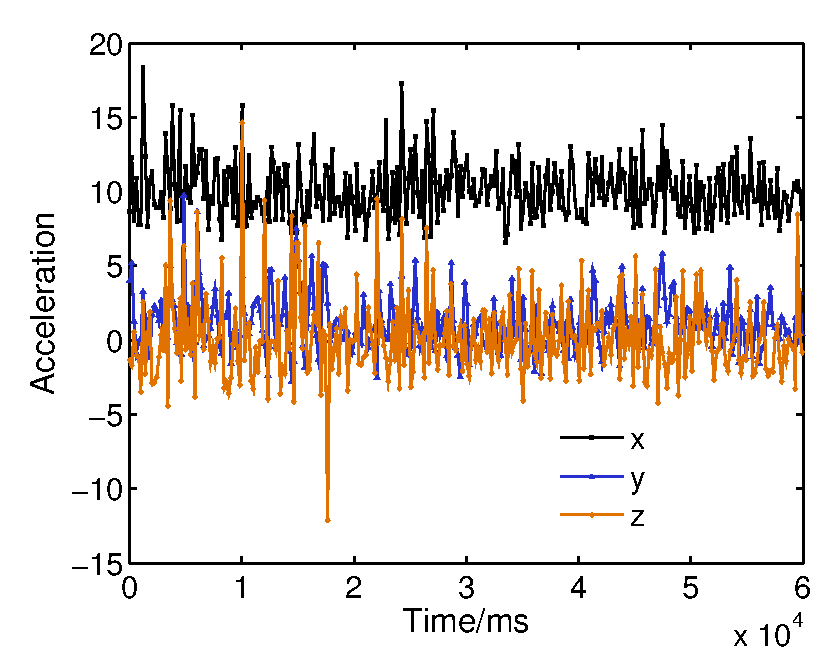
\includegraphics[height=40mm]{fig/good_raw.eps}
    \caption{Example of a good sequence from raw data: samples points are close in time. These points are regarded as representing a single activity.}
    \label{fig:good_raw}
    \end{minipage}
    \begin{minipage}[t]{0.02\textwidth}~
    \end{minipage}
    \begin{minipage}[t]{0.47\textwidth}
    \centering
    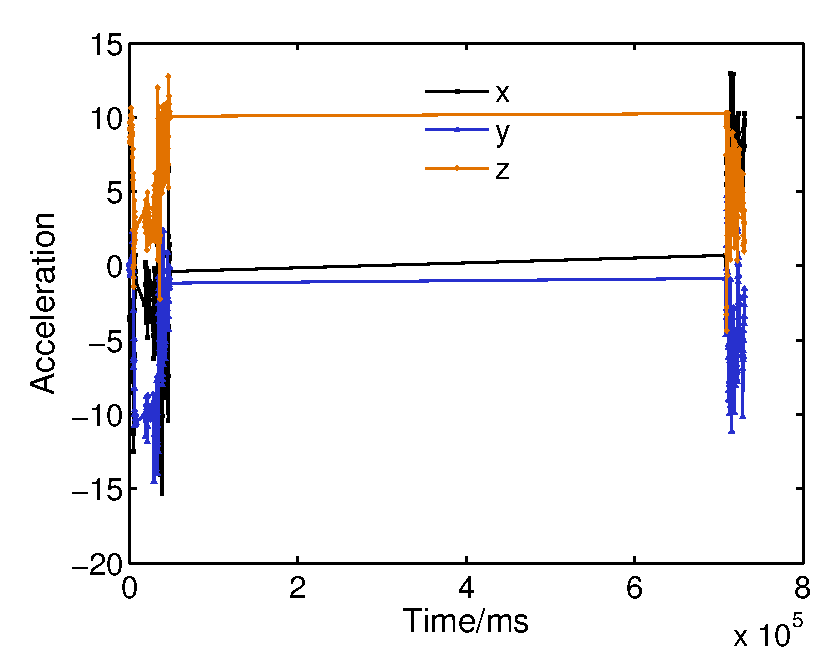
\includegraphics[height=40mm]{fig/bad_raw.eps}\\
    \caption{Example of a bad sequence from raw data. This piece essentially contains information about two separate activities that are far apart in time. The line segments in the middle of the figure was due to the large time intervals between adjacent sample points.}
    \label{fig:bad_raw}
    \end{minipage}
    \begin{minipage}[t]{0.02\textwidth}~
    \end{minipage}%   
 \end{figure}


\paragraph{Segmentation} % (fold)
For each sequence of samples in the raw data, the time intervals between two adjacent sample points are less than 500 ms for most of the time. However, some intervals can be as large as 100,000 ms. This is illustrated in Figures \ref{fig:good_raw} and \ref{fig:bad_raw}. In the first sequence, all  points are close in time, and they can be treated as representing a single activity. In the second, there are two points with a large time difference. Thus, we can consider this sequence containing information about two separate activities. It is clear that we cannot process this sequence as a whole. %This could be attributed to two 

To tackle this, a two-phase segmentation was performed. First, the sequences with time intervals larger than $T_\mathrm{split}$ were split, resulting in several subsequences for each original sequence. Second, we continually split the longest subsequence among all the subsequences until 1) we got $k_\mathrm{\#seq}$ subsequences, or 2) the longest one was shorter than $2 l_\mathrm{maxL}$. Also, sequences shorter than $T_\mathrm{short}$ were thrown. After segmentation, on the one hand, we make more sequences from one device, hopefully keeping more information about the device's diverse patterns. On the other hand, we keep the sequences long enough, so that they contain reliable information about patterns of the user.

\paragraph{Re-sampling} 
After segmentation, for each device, we got several subsequences. However, these sequences were not uniformly sampled, due to various reasons. To make feature extraction simpler, we interpolated each segment using cubic spline and uniformly re-sampled each sequence with  $\tau_\mathrm{resample}$ being the re-sampling time interval.

\subsection{Feature extraction}
\label{feautures}

After preprocessing, for each raw sequence (from training set or testing set), we got several shorter re-sampled subsequences. In this section, we describe how to extract features from each subsequence. Six categories of features were investigated. They represent different aspects of patterns from the data.

\paragraph{Frequency domain features}
As different people has their own pace for actions, we believe the patterns of human mobility can be easily exploited in frequency domain. To this end, for each subsequence, we first extracted sliding windows of size $w_\mathrm{fft}$ and 50\% overlap (features extraction on windows with 50\% overlap has demonstrated success in previous work \cite{Bao:PC2004}). Then we did FFT on all windows. Finally, we calculated the magnitude of all first $(w_\mathrm{fft}/2 + 1)$ coefficients and used the average values over all windows as the frequency domain features for the subsequence. Because readings were from 3 directions, we have $(w_\mathrm{fft}/2 + 1)\times 3$ values for frequency domain features per subsequence.

\paragraph{Differences of acceleration}
More patterns and properties were discovered when we look beyond frequency domain. One obvious feature is the absolute difference between two adjacent readings of acceleration \cite{Kwapisz:BTAS2009}. This feature measures how rapidly a person usually handles the phone or moves. It may also indicate the environment this person lives. The distribution of such differences was taken as the features in this category. Specifically, we computed three histograms (30 bins each histogram, edges of leftmost and rightmost bins determined by the 5\% and 95\% quantiles of absolute differences for each axis) of absolute differences between every adjacent pair of readings on three axes for each sequence as its features. 

\paragraph{Resultant acceleration}
The value of each reading alone can also imply useful information. The resultant acceleration \cite{Kwapisz:BTAS2009}, which is defined as $\sqrt{x^2+y^2+z^2}$ ($x,y,z$ are readings at a particular time), directly evaluates the absolute value of the acceleration of the device. This value reveals how hard a person usually moves as the force is proportional to the acceleration it measures. The distribution of resultant acceleration is the third feature we used. Same as mentioned above, the histogram (prepared in the same way as the previous feature) of this value was produced for each sequence as one category of its features.

\paragraph{Histogram of acceleration readings}
Inspired by the above features, distribution of acceleration readings each of three dimensions can also be informative. For example, a phone may lie on a desk if the reading of its reading for z axis (the axis perpendicular to the screen) is more likely to be 9.8 $\mathrm{m}\cdot \mathrm{s}^{-2}$ (gravity), while another phone's reading for y axis is larger when it is always kept in one's pocket. Three histograms (prepared in the same way as the previous two features) were generated for every sequence.

The above four sets of features were what we mainly focused on. There were also many tricky features which could help us a lot to have a better score in the competition. However, these features could be useless in real world applications. 

\paragraph{Raw sampling rate}
As the mobile devices people use are increasingly diverse, the characteristics of different devices offer us a set of very distinguishing features for recognizing users. One of these characteristics was the sampling intervals of the devices.

As we observed from the raw data set, sampling intervals of devices has a range of approximately 5-250 ms, and for different devices, the distributions of the sampling intervals were quite different. Thus, for each subsequence, we used the histogram (0-600 ms divided into bins of 20 ms, in total 30 values) of the sampling intervals of the original sequence it came from as the time domain features. 

\paragraph{Sampling granularity}
Apart from the sampling intervals of devices, we found another set of features with potential ability of distinguishing devices, which was the accelerometer readings.

By observing the data, we found that each kind of device could only provide certain discrete values of accelerometer readings, and this might be due to the limited precision of accelerometers. Thus, the set of accelerometer readings a device can provide is also treated as a set of features. For each subsequence, we calculated the overlap between the the set of readings from the original sequence it came from and the set of readings from the $i$th device, $i=1,\ldots,387$. Since we had readings from 3 directions, $3\times 387 = 1161$ values constituted the accelerometer reading features for each subsequence.

The two tricky features introduced above help teams to gain satisfactory scores in the Kaggle competition. However, they focus more on classifying devices rather than users. They could easily fail in real world when a large amount of people use the same type of devices such as iPhones. These features may also fail when a person uses several devices at the same time or switches to a new device.

\subsection{Classification}

Once the key features are extracted, we move on to leverage various kinds of classifiers and optimize their parameters for more accurate results.

After preprocessing and feature extraction, for each original sequence, we now had several feature vectors associated with it. These vectors were used for classification. For each vector, we let the classifier output the probability (belief) that it comes from device $i$ ($i=1,\ldots,387$). Then, the average of beliefs of all feature vectors associated with a test sequence on the proposed DeviceId was used for submission.

We started from some naive classifiers. The performance of K-nearest-neighbor depends on the number of K and the definition of distance function. This classifier gave us a baseline result. Then we moved on to popular classifiers such as support vector machines and logistic regression. We also investigated the impact of the parameters of these classifiers in the following sections about implementation.


\section{Implementation and Evaluation}
In this section we show how our approach performed. We will justify the selection of parameters for preprocessing. We will also show the impact of quantity of training data and different features on results. We hope this could tell us how much training data is required to achieve an acceptable performance, and more importantly, how to prevent leakage of our identity by controlling what kind of accelerometer data to use.

\subsection{Evaluation methods and metrics}
We used the online judging system of Kaggle for fairness. It could also demonstrate how our approach performed against other teams all over the world. 

The system took results generated from our classifier as input. Then, the system produced value of area under the ROC curve (AUC) as the score. The baseline of AUC is 0.5 which stands for purely random guesses. A higher AUC value means a better classifier. A result with AUC of 1 stands for perfect guess. 

\subsection{Parameter selection}
In this subsection we discuss how to determine the parameters and thresholds we defined in the previous sections.


\subsubsection{Preprocessing}
$T_\mathrm{split}$ was set to be 10 seconds to be consistent with the preprocessing setting done by Kaggle.  $T_\mathrm{short}$ and $l_\mathrm{maxL}$ were both set to be 4.8 seconds for the training set and 3.2 seconds for the testing set empirically. $\tau_\mathrm{resample}$ was set to be 200 milliseconds based on statistics of the distribution of the time intervals of the raw data, but any value near 200 ms should be a reasonable choice. The window size of FFT, $w_\mathrm{fft}$, was 64, which meant a window of duration 12.8 seconds. For training, $k_\mathrm{\#seq}=50$; for testing, $k_\mathrm{\#seq}=5$.

\subsubsection{Frequency domain granularity}
One of the important parameters is the number of samples for FFT. The re-sampling was taken at 200ms. So, FFT features describes the data's frequency components from 0Hz to 1/0.2/2 = 2.5Hz. With original 64 point FFT, the frequency components are spaced at 2.5/32 Hz. 

However, such fine granularity in frequency domain (2.5/32 Hz between components) may not necessarily lead to better results. Some of these components can be highly correlated and so be redundant and even lead to worse performance. We wanted to investigate how the granularity of these features affect the performance. To do this, we first did 96 point FFT (48+1 features per axis) and 64 point FFT (32+1 features per axis) on each sequence. Then we down-sampled these features by only keeping every 2-, 4-, 8-, and 16-th components, so that we had 10 different sets of FFT features for each sequence, covering the frequency from 0Hz to 2.5Hz, but at different granularities.


\begin{figure}
    \hspace{-0.5cm}
    \begin{minipage}[t]{0.02\textwidth}~
    \end{minipage}
    \begin{minipage}[t]{0.47\textwidth}
    \centering
    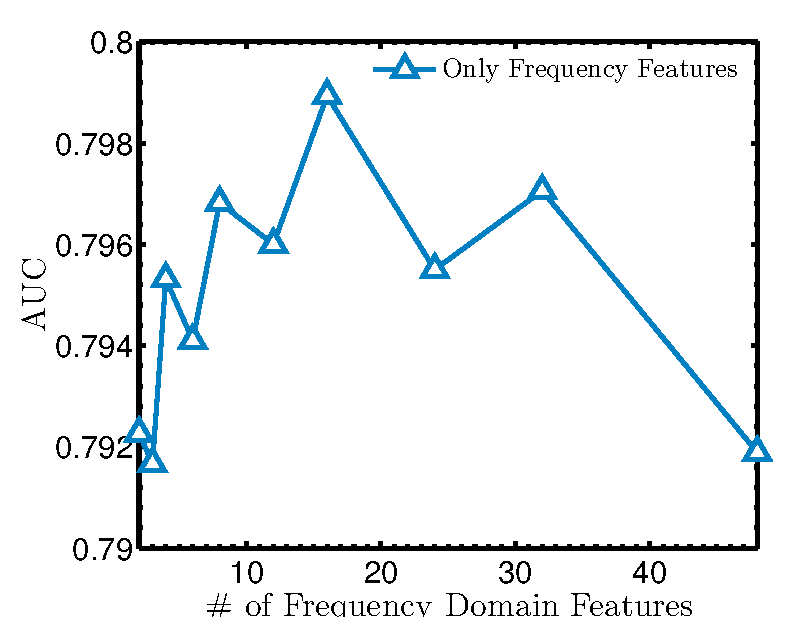
\includegraphics[height=40mm]{fig/fftauc.eps}
    \caption{AUC vs granularity of features in frequency domain. Only frequency domain features are used with logistic regression.}
    \label{fig:FFTAUC}
    \end{minipage}
    \begin{minipage}[t]{0.02\textwidth}~
    \end{minipage}
    \begin{minipage}[t]{0.47\textwidth}
    \centering
    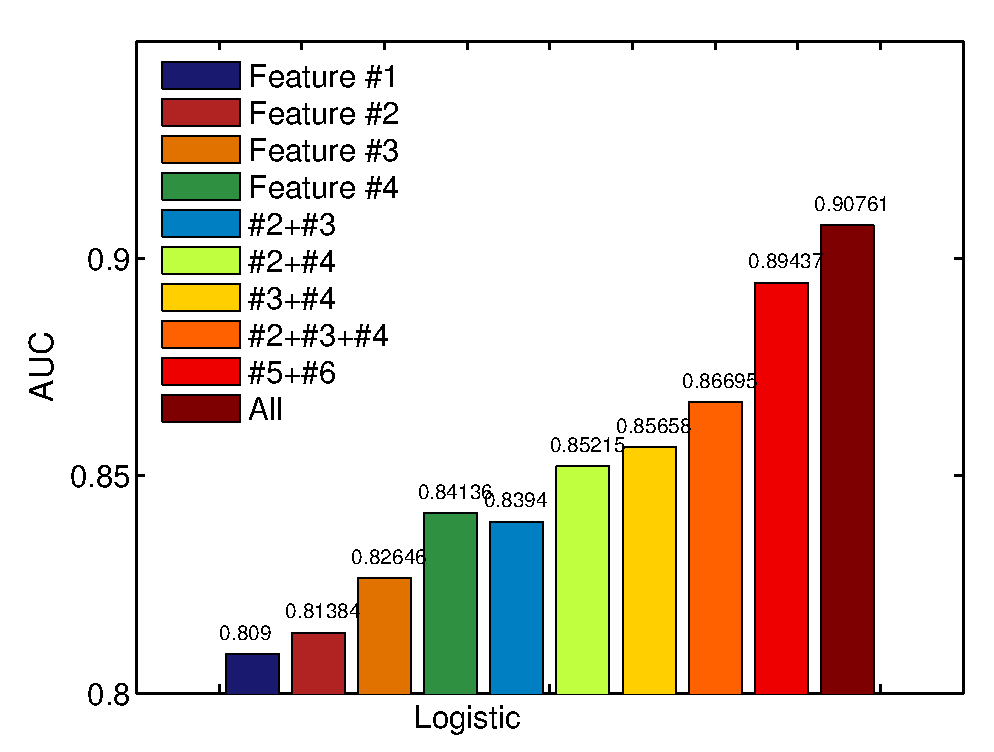
\includegraphics[height=40mm]{fig/feature}\\
    \caption{AUCs vs combinations of features using logistic regression.}
    \label{fig:feature}
    \end{minipage}
    \begin{minipage}[t]{0.02\textwidth}~
    \end{minipage}%   
 \end{figure}

Figure \ref{fig:FFTAUC} shows the results for different frequency granularities. We only applied frequency domain features on logistic regression. The result indicates that feature vectors of length 17 to 33 perform better than smaller or greater ones on average. We can also find that neither smaller nor larger number of features performed significantly worse than the optimal ones. This fact means fine-grained feature extraction cannot exploit much more independent features than the coarse-grained ones. The reasons could be: 1) patterns of human movement do not have strong regularity on the frequencies (0 Hz to 2.5 Hz) we investigated. 2) accelerometer is not sensitive enough to gather that many useful features. 3) the features there are useful in theory, but noise due to accelerometer and other factors is also strong in that frequency range. If we have devices better than cellphone in terms of sensitivity and noise reduction, we may better explain this phenomenon.

Since there was no substantial difference for choices of granularity, in the following experiments, we just used 3 features (the shortest among all feature vectors we tested) for each axis as FFT features (also known as ``Feature \#1'').

\subsection{Tuning classifier}
Our preliminary results showed that L2-norm K-nearest-neighbor algorithm ($k=40$) leads to really poor results which achieved less than 0.6 in AUC. Although $k$ and the metric could be changed, we simply abandoned KNN for its poor performance and its time-consuming computation.

We use logistic classifier as one of our main options. The only parameter can be tuned in this classifier is $C$ (in LIBLINEAR) as the regularization parameter of logistic regression. It turns out that our features and data were not sensitive to the value of $C$ (no matter what combination of features used, AUC only fluctuated by about 0.0002). Therefore, we just used $C=1$.

We also tried support vector machine classifier. As it was very time-consuming, we only tested $C=1, \gamma=1$ (LIBSVM) for a SVM with a Gaussian kernel.

\subsection{Results}

Here we present the performance of our classifiers. For convenience, we denoted 6 kinds of features used as Feature \#1 to Feature \#6, corresponding the order they appear in the section of feature extraction. First, we show the performance of classifiers using all 6 features. Second, results for different combinations of features are given. Last, results under different amounts of training data are shown.

\paragraph{All features} % (fold)
\label{ssub:all_features}
Here, all resuls on reported using all 6 kinds of features, in Table \ref{tbl:test_result}.
% subsubsection all_features (end)

\begin{table}[!ht]
\caption{AUCs for different classifers, using all kinds of features}
\label{tbl:test_result}
	\begin{center}
		\begin{tabular}{ c | c  c  c  }
			\hline
			 Methods & L2-norm KNN & SVM & LR \\
			 \hline
			 AUC & 0.58302 & 0.80701 & \textbf{0.90761} \\
			 \hline
		\end{tabular}
	\end{center}
\end{table}


\paragraph{Combinations of features} % (fold)
\label{ssub:combinations_of_features}
Results using different combinations of features are reported in Figure \ref{fig:feature}. Only logistic regression was used for classification.

% subsubsection combinations_of_features (end)


\paragraph{The impact of amount of training data on performance} % (fold)
\label{ssub:the_impact_of_amount_of_training_data_on_performance}
Results using different amounts of training data are shown in Figure \ref{fig:percentage}. We reduce the size of training data by randomly selecting a portion of all training feature vectors, each vector corresponding to a split and re-sampled subsequence. Note that because Features \#5 and \#6 were not generated based on the subsequence, only Features \#1 to \#4 were used in this test. Again, only logistic regression was used.

\begin{figure}
    \centering
    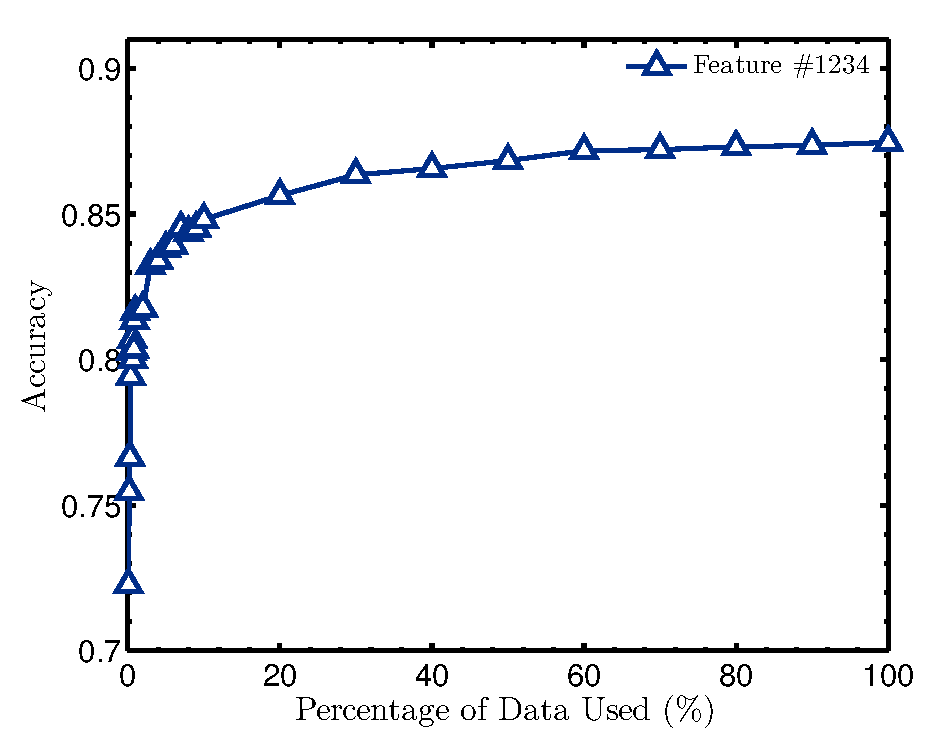
\includegraphics[height=40mm]{fig/percentage.eps}\\
    \caption{AUCs vs percentage of training data using logistic regression.}
    \label{fig:percentage}
 \end{figure}

% subsubsection the_impact_of_amount_of_training_data_on_performance (end)
\paragraph{Miscellaneous results using SVM}  % (fold)
\label{subs:miscellaneous}
Because using SVM was very time-consuming, we only tested under several conditions, and the results are shown in \ref{tbl:test_result_SVM}.

\begin{table}[!ht]
\caption{AUCs for different conditions, using SVM}
\label{tbl:test_result_SVM}
    \begin{center}
        \begin{tabular}{ c | c  c  c  }
            \hline
             Features & All & only \#1 & \#1 + \#2 + \#3 +\#4 (10\% training data) \\
             \hline
             AUC & 0.80701 & 0.81406 & \textbf{0.85112} \\
             \hline
        \end{tabular}
    \end{center}
\end{table}

% subsection miscellaneous (end)

\subsection{Analysis} % (fold)
\label{sub:analysis}

% subsection analysis (end)

The best result from our approach ranked top 8\% out of 634 teams on Kaggle. Although, the top teams reach over 0.99 of AUC for this competition, the tricky features mentioned in previous section boost the accuracy a lot. According to the online discussion, simply using tricky features to distinguish and identify sensors could achieve the ideal results. This was also partially proved by our result using Features \#5 and \#6 in \ref{fig:feature}, which is just a little behind the result using all features. When using all features, clearly logistic regression was far better than other options. Although the parameter of SVM wasn't thoroughly tuned due to time limit, we tried some parameters of SVM and empirically they didn't make significant improvement for SVM. K-nearest-neighbor was the worst of all three, and we didn't work on that any more, again, because tuning it was time-consuming and seemed hopeless to improve the result.

The results in Figure \ref{fig:feature} may suggest two things. 1) Histogram features (\#2-\#4) are more informative than FFT features (\#1) in this task, and they are also ``safer'' (see next section for detail) in terms of protecting user's real trajectory. 2) Tricky features (\#5, \#6) are very useful in this competition, but its usefullness in reality may be limited, e.g. when all devices are the same or very similar.


The results in Figure \ref{fig:percentage} suggest two things. 1) The training dataset provided by Kaggle is somewhat redundant, since in the range from 30\% to 100\%, there was only a slight and gradual decrease in accuracy. 2) We don't need too much data or time for this task, since emperically there was no much difference between the performance using 20\% data and the one using all data, and training can be done rather quickly (it only took about 10 seconds to train 20\% of all training data on a 12-core server), making training on mobile devices possible. Note that these results were generated based on only one random selection of training data, so there's sampling error in it, but we think the general relationship between performance and amount of training data should not change if more random selections were done.

Results in Table \ref{tbl:test_result_SVM} were just a partial evluation of SVM for this task. However, two things seem true. 1) With high-dimensionality feature vectors (all 6 kinds of features), SVM with Gaussian kernel seemed to perform a lot worse than linear methods (0.80701 using SVM vs. 0.90761 using LR). 2) SVM with Gaussian kernel seems to perform better than linear methods with shorter feature vectors and smaller data set (0.85112 using SVM vs. 0.84816 using LR, using Feautures \#1 to \#4 and 10\% of data).

Although the competition became a game of cheating as it suffers from ``leaks'', as quoted from one of the best teams, we, who did not take effort to leverage leaks, show that reasonable features, which are obtainable in real world, also lead to promising results.


\section{Privacy Control}
In this section we look beyond the competition for a more practical issue, privacy. By saying protecting user privacy, we mean that identifying users without revealing users' activity (the trajectory of the acceleration readings), e.g.\ what the user did at 6pm of Dec. 10, 2013, and device type. The idea is similar to the fingerprint technology in the iPhones, where fingerprints are collected as an identification but not stored or revealed to others, using a hashing process.

To protect user privacy, features which may cause privacy leak were eliminated (including Feature \#1 which can be used to reconstruct the original acceleration data and Feature \#5 and \#6 which may reveal device type). We assume that histogram features (Features \#2 to \#4) are safer than the frequency domain features. The reason is that the FFT features may be still invertible to original time domain readings while it is much harder to recovery the time domain trace from histograms.


Classification performance was tested on using all features against using Features \#2 to \#4 using the best performing logistic regression classifier. As shown in Figure~\ref{fig:feature}, comparable results were gained by restricted features. The classifier using only Features \#2 to \#4 got 0.867 AUC compared to the 0.908 AUC got from all features. Thus, using our classifier with restricted features, we can have satisfactory identification accuracy while protecting users' privacy.

However, we noticed that even when we use just Features \#2 to \#4, we are facing the risk of privacy leak because features like the difference of acceleration or distributions of acceleration may to some extent reveal user's activity (trajectory). For example, a sequence of acceleration sampled when a user is sitting will certainly have acceleration distributions differing from that of one sampled when the user is running. Also we noticed that, device dependent features (Features \#5 and \#6) were very successful in this competition (Figure~\ref{fig:feature}). Although these feature can only reveal device type, it is still possible that these information may compromise privacy.

Here are some possible ways to further protect user privacy: 1) Applying certain hashing technologies (e.g.\ locality-sensitive hashing) to the features extracted from the raw data will be helpful for protecting privacy. 2) It would be helpful if the mobile phone manufacturers can perform ``normalization'' on the output of accelerometers and even other sensors based on one standard. Having a standard output form can prevent the leakage of the type of device users have.

\section{Conclusion and Future Work}


We have learned a few things from this project besides a better understanding of machine learning itself as our classifier identifies users well. First, the assumption that human beings have patterns of movement is true. Second, both time domain and frequency domain features help this technique. Third, we have the preliminary knowledge of how to control the leakage of acceleration data to protect our privacy against such technique. By limiting type of features used, protection can be achieved. Furthermore, we believe that applications such as anti-theft, health monitoring and emergency detection that adopt this novel identification technique will be available in the near future.

We could have better results and studies if we get more time in this project. First, the SVM classifier could be tuned more. Second, as we have known that the dataset is somewhat redundant, we can train more classifers using different portions of the training data and do some kind of model combination (e.g. boosting) to improve the result. What's more, if we have a device more sensitive and less noisy than cellphone, we could further study the patterns of movement and their effectiveness. At last, we are hoping to build a software framework or library for such technique so that it could be available for practical usage.


\bibliographystyle{IEEEtranS}
\bibliography{references}



\end{document}
